%%%%%%%%%%%%%%%%%%%%%%%%%%%%%%%%%%%%%%%%%
% a0poster Portrait Poster for LiRI/UZH
% LaTeX Template
% Version 1.0 (22/06/13)
% Version 2.0 (08/04/22)
%
% The a0poster class was created by:
% Gerlinde Kettl and Matthias Weiser (tex@kettl.de)
% adapted by Danny McDonald for LiRI/UZH (mcddjx@gmail.com)
%
% License:
% CC BY-NC-SA 3.0 (http://creativecommons.org/licenses/by-nc-sa/3.0/)
%
%%%%%%%%%%%%%%%%%%%%%%%%%%%%%%%%%%%%%%%%%

\documentclass[a0,portrait]{a0poster}

% control margins here
\usepackage{geometry}
 \geometry{
 a0paper,
 left=5cm,
 top=4.5cm,
 right=5cm,
 bottom=4.5cm
 }
\addtolength{\textwidth}{4.5cm} % width of text can be adjusted if margins above are adjusted

\usepackage{multicol} % This is so we can have multiple columns of text side-by-side
\columnsep=3em % This is the amount of white space between the columns in the poster
\columnseprule=0pt % This is the thickness of the black line between the columns in the poster

% UZH colours
\usepackage[svgnames]{xcolor}
\definecolor{uzhblau100}{RGB}{0, 40, 165}
\definecolor{uzhblau80}{RGB}{51,83,183}
\definecolor{uzhockerrot100}{RGB}{220, 96, 39}
\definecolor{uzhockerrot80}{RGB}{227, 128, 82}
\definecolor{uzhflaschengruen100}{RGB}{42, 127, 98}
\definecolor{uzhflaschengruen80}{RGB}{86, 157, 133}
\definecolor{conclusion}{RGB}{204,212,237} % the conclusion box colour

\usepackage{ifthen} % needed to stop horizontal line above 'Conclusions' section
\usepackage{graphicx} % Required for including images
\graphicspath{{img/}} % Location of the graphics files
\usepackage{mwe,tikz}\usepackage[percent]{overpic} % overlay your photo over the background
\usepackage{booktabs} % Top and bottom rules for table
\usepackage[font=small,labelfont=bf]{caption} % Required for specifying captions to tables and figures
\usepackage{amsfonts, amsmath, amsthm, amssymb} % For math fonts, symbols and environments
\usepackage{wrapfig} % Allows wrapping text around tables and figures

\usepackage{fontspec} % custom fonts
\defaultfontfeatures[Palatino]
{
    Extension = .ttf,
    UprightFont = font/LT_41167,
    BoldFont = font/LT_41169,
    ItalicFont  = font/LT_41168,
    BoldItalicFont = font/LT_41170,
}
\defaultfontfeatures[TheSans]
{
    Extension = .otf,
    UprightFont = font/TheSans-LP5Plain,
    BoldFont = font/TheSans-LP7Bld,
    ItalicFont  = font/TheSans-LP5PlainIT,
    BoldItalicFont = font/TheSans-LP7BldIT,
}
\setmainfont{TheSans} % choose your font here
\usepackage[onehalfspacing]{setspace} % remove for single spacing
\usepackage{tcolorbox} % for the conclusions box
\usepackage{blindtext} % you can remove this once you add your content
\usepackage[export]{adjustbox} % allow floating a graphic right
\usepackage{titlesec} % customising section titles
\usepackage{needspace} % prevent break between line and section title
\usepackage{nameref} % package and command to get the name of the current section (for ifthen)

\begin{document}

% define how our section titles will look (with ruled line)
\titleformat{\section}
  {\needspace{1\baselineskip}\sectionrule\huge\bfseries}
  {\color{uzhblau100}\thesection.}
  {1em}
  {\color{uzhblau100}}

% draw horizontal line before section unless it is conclusions (if you change name of Conclusions, you should
% also change it here too so it is recognised and the line suppressed
\makeatletter
\newcommand{\sectionrule}{%
 \ifthenelse{\equal{\@currentlabelname}{Conclusions}}
 % use the below line instead of the above if conclusions is a section*
 % \ifthenelse{\equal{\@currentlabelname}{}}
  {}
  {\vspace*{-\baselineskip}
   \vrule height 1pt depth 1pt width \linewidth\vskip0.4pt
   \bigskip}%
}
\makeatother


%----------------------------------------------------------------------------------------
%	POSTER HEADER 
%----------------------------------------------------------------------------------------
%\title{Creating a \LaTeX{} poster template matching UZH specifications for LiRI presentations}
\title{Titel zum Thema des Posters: Lesbar aus fünf Metern Distanz  und eindeutig formuliert}

% the top logo (in english!) and unit title
\noindent
\begin{minipage}{.32\linewidth}
 
\includegraphics[width=20cm]{logoCPNV.png}
\end{minipage}%
\begin{minipage}{.33\linewidth}
 \huge{\textbf{Linguistic Research Infrastructure}}
\end{minipage}
\vspace{4em}

% The header is divided into two boxes, on the left is the text and on the right is the image
\begin{minipage}[b][][t]{.6\linewidth}
\vfill
\makeatletter
\raggedright{\fontsize{92pt}{100pt}\selectfont\color{uzhblau100}\textbf{{\@title}}\par}
\makeatother
\color{Black}
\vspace{1cm}
%\Huge\textit{Subtitle goes here}\\[2.4cm] % Subtitle if it exists
\underline{Danny McDonald\textsuperscript{1}}, Autor Zwei, Autor Drei\\
\vspace{0.2cm}
\textsuperscript{1}LiRI, University of Zurich
%\\ % add your institution
%\texttt{you@uzh.ch}%\\ % add your email
\end{minipage}%
%
\begin{minipage}[b][][t]{0.39\linewidth}
\vfill
  \begin{overpic}[width=.8\textwidth,right]{logoMCT.jpg} % what even is this thing?
     \put(85,0){
\includegraphics[scale=0.25]{logoCPNV.png}}  % your image goes in here
  \end{overpic}
\end{minipage}
\vspace{1cm}

%----------------------------------------------------------------------------------------
%	POSTER BODY
%----------------------------------------------------------------------------------------

\begin{multicols}{3} % This is how many columns your poster will be broken into

%----------------------------------------------------------------------------------------
%	INTRODUCTION
%----------------------------------------------------------------------------------------

\section{Untertitel}

\large
Fliesstext mit einfachem Satzbau und kurzen Hauptsätzen erleichtern die Lesbarkeit. Lorem ipsum dolor sit amet, consectetuer adipiscing elit. Aenean commodo ligula eget dolor. Aenean massa. Cum sociis natoque penatibus et magnis. Donec quam felis, ultricies nec, pellentesque eu. Aenean commodo ligula eget dolor. Aenean massa.

\begin{itemize}
\item An example of a bullet point
\item A second example of a bullet point, this one taking up more than one line just to see how it displays
\item Third, short point
\end{itemize}
\blindtext
\begin{center}
 \vspace{2cm}
 \begin{tabular}{c c c c} 
  \toprule
  Col1 & Col2 & Col2 & Col3 \\ [0.5ex] 
  \midrule
  1 & 6 & 87837 & 787 \\ 
  2 & 7 & 78 & 5415 \\
  3 & 545 & 778 & 7507 \\
  4 & 545 & 18744 & 7560 \\
  5 & 7 & 78 & 5415 \\
  6 & 545 & 778 & 7507 \\
  \bottomrule
 \end{tabular}
\captionof{table}{A dummy table in the centre of the column}
\vspace{2cm}
\end{center}

%----------------------------------------------------------------------------------------
%	SECTIONS
%----------------------------------------------------------------------------------------

\section{Next section}
\blindtext

\begin{center}\vspace{1cm}
    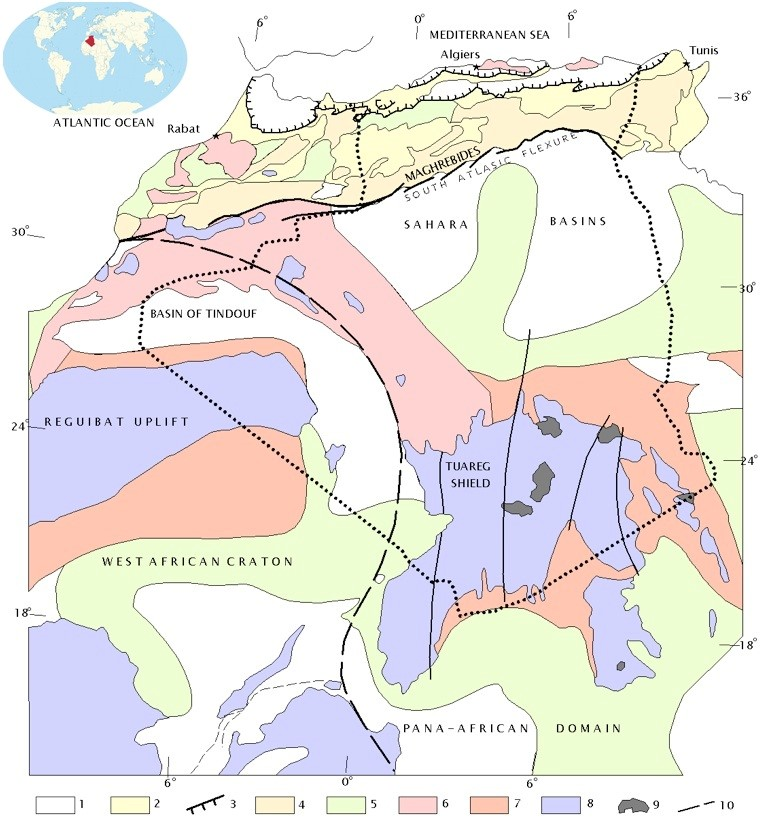
\includegraphics[width=0.8\linewidth]{Figure_1}
    \captionof{figure}{Regional map with some colours}
\end{center}\vspace{1cm}

%----------------------------------------------------------------------------------------
%	CONCLUSIONS BOX
%----------------------------------------------------------------------------------------

%\section*{} % this dummy section draws a horizontal line above conclusions
\vspace{2cm}
\begin{tcolorbox}[width=0.95\linewidth,colback={conclusion},frame empty,boxsep=1cm]
\section{Conclusions}
\blindtext
\end{tcolorbox}    

%----------------------------------------------------------------------------------------
%	FORTHCOMING RESEARCH
%----------------------------------------------------------------------------------------

\section{Forthcoming Research}

\blindtext
\color{uzhockerrot100}
\begin{itemize}
 \item An example of a bullet point in UZH highlight colour
 \item A second example of a bullet point, this one taking up more than one line just to see how it displays
 \item Third, short point
\end{itemize}
\color{Black}

%----------------------------------------------------------------------------------------
%	REFERENCES
%----------------------------------------------------------------------------------------
\singlespacing
\small
\nocite{*} % Print all references regardless of whether they were cited in the poster or not
\bibliographystyle{plain} % Plain referencing style
\bibliography{sample} % Use the example bibliography file sample.bib

%----------------------------------------------------------------------------------------

\end{multicols}
\end{document}